\documentclass[../notes.tex]{subfiles}

\pagestyle{main}
\renewcommand{\chaptermark}[1]{\markboth{\chaptername\ \thechapter\ (#1)}{}}
\setcounter{chapter}{3}

\begin{document}




\chapter{Spectroscopy Wrap-Up}
\section{XPS and Misc. Spectroscopic Techniques}
\begin{itemize}
    \item \marginnote{1/24:}If it looks like there will be snow on exam day, we'll do a virtual exam.
    \item The exam is open notes, but we can do cameras on or something like that.
    \item Submit the HW any time before the exam to both Shevchenko's anl.gov and uchicago.edu addresses; put "Homework" in the subject line.
    \item We now start the lecture, picking up from last time on TEM.
    \item TEM back then.
    \begin{itemize}
        \item High-voltage electron microscopy was developed in 1968, even though this is antiquated by today's standards.
        \item The idea is that this high-voltage one (megavolt range) produced electron beams $10\times$ as strong.
        \item Check out \emph{cite}; it was the state of the art back then.
        \item Where has this slide gone??
    \end{itemize}
    \item Interaction of electrons with matter.
    \begin{itemize}
        \item Reviews Figure \ref{fig:ElectronsMatter}.
        \item TEM utilizes the transmitted electrons (both elastically and inelastically scattered).
    \end{itemize}
    \item Conventional TEM (CTEM).
    \begin{figure}[H]
        \centering
        \begin{subfigure}[b]{0.49\linewidth}
            \centering
            \begin{tikzpicture}
                \small
                \fill [gray!30] (-3,-0.2) rectangle (3,0.2);
                \node [right] at (3,0) {Specimen};
        
                \footnotesize
                \draw [thick,-latex] (0,1.3) node[above]{Incident electrons} -- (0,0.3);
        
                \draw [semithick,-latex] (0,-0.3) -- (1.2,-1.5) node[below right,text width=1.7cm]{Elastically scattered electrons};
                \draw [semithick,-latex] (0,-0.3) -- (0,-3) node[below,align=center]{{\color{blx}Transmitted electrons}\\{\color{blx}(and electrons scattered at low angles)}};
                \draw [semithick,-latex] (0,-0.3) -- (-1,-1.7) node[below left,text width=1.7cm,align=right]{Inelastically scattered electrons};
        
                \filldraw [fill=blx]
                    (-2,-1) rectangle (-0.2,-0.9)
                    (0.2,-1) rectangle (2,-0.9) node[above,xshift=5mm]{\small Objective lens aperture}
                ;
        
                \path (-4,0) -- (4.5,0);
            \end{tikzpicture}
            \caption{Bright field.}
            \label{fig:brightDarkOLa}
        \end{subfigure}
        \begin{subfigure}[b]{0.49\linewidth}
            \centering
            \begin{tikzpicture}
                \small
                \fill [gray!30] (-3,-0.2) rectangle (3,0.2);
                \node [right] at (3,0) {Specimen};
        
                \footnotesize
                \draw [thick,-latex] (0,1.3) node[above]{Incident electrons} -- (0,0.3);
        
                \draw [semithick,-latex] (0,-0.3) -- (1.2,-1.5) node[below right,text width=1.7cm]{{\color{grx}Elastically scattered electrons}};
                \draw [semithick,-latex] (0,-0.3) -- (0,-3) node[below,align=center]{Transmitted electrons\\{\color{white}(and electrons scattered at low angle)}};
                \draw [semithick,-latex] (0,-0.3) -- (-1,-1.7) node[below left,text width=1.7cm,align=right]{Inelastically scattered electrons};
        
                \filldraw [fill=grx]
                    (-2,-1) rectangle (0.45,-0.9)
                    (0.85,-1) rectangle (2,-0.9) node[above,xshift=5mm]{\small Objective lens aperture}
                ;
        
                \path (-4,0) -- (4.5,0);
            \end{tikzpicture}
            \caption{Dark field.}
            \label{fig:brightDarkOLb}
        \end{subfigure}
        \caption{OL configuration in bright and dark field modes.}
        \label{fig:brightDarkOL}
    \end{figure}
    \begin{itemize}
        \item You don't often see "CTEM" (usually just "TEM").
        \item The sample is illuminated with electrons.
        \begin{itemize}
            \item Only the ones that pass through the specimen are used.
        \end{itemize}
        \item The direct image is formed by the objective lens and is recorded in the image plane.
        \item Two modes: \textbf{Bright field} and \textbf{dark field}.
    \end{itemize}
    \item \textbf{Bright field}: Some areas of the sample absorb electrons and appear darker, while other areas that transmit electrons appear brighter. The transmitted electron beam is selected with the aperture, and the scattered electrons are blocked.
    \item \textbf{Dark field}: The transmitted electrons are excluded from the aperture, and the scattered electrons are selected. The areas where there is no electron scattering (e.g., the areas around the sample) will be black.
    \begin{itemize}
        \item The main difference between the two modes is which electron populations are used to construct the TEM image.
    \end{itemize}
    \item Bright field and dark field TEM micrographs.
    \begin{figure}[h!]
        \centering
        \begin{subfigure}[b]{0.3\linewidth}
            \centering
            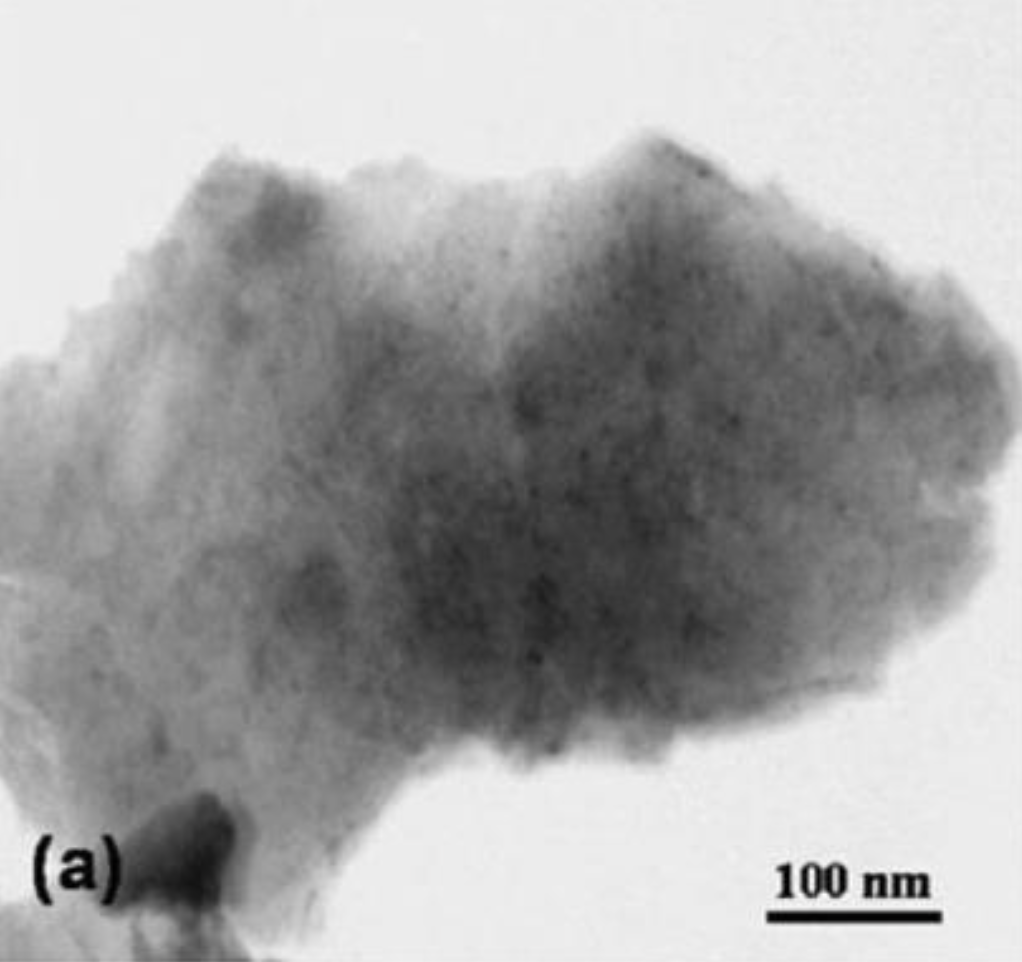
\includegraphics[width=0.8\linewidth]{BrightDarkMicrographa.png}
            \caption{Bright field.}
            \label{fig:BrightDarkMicrographa}
        \end{subfigure}
        \begin{subfigure}[b]{0.3\linewidth}
            \centering
            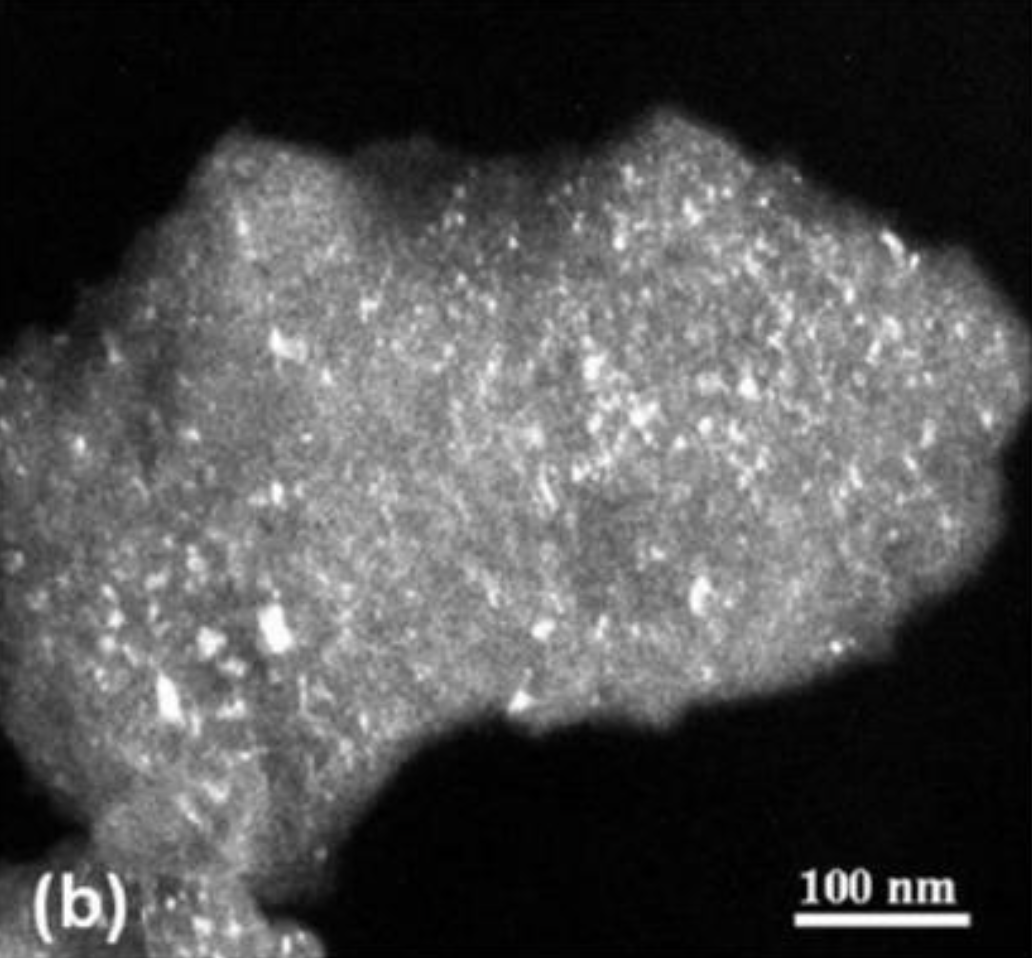
\includegraphics[width=0.8\linewidth]{BrightDarkMicrographb.png}
            \caption{Dark field.}
            \label{fig:BrightDarkMicrographb}
        \end{subfigure}
        \caption{Bright field and dark field TEM micrographs.}
        \label{fig:BrightDarkMicrograph}
    \end{figure}
    \begin{itemize}
        \item Can be used to study crystal lattices, crystal defects, stacking faults, dislocations, and particle/grain sizes.
        \item Basic observations.
        \begin{itemize}
            \item Bright: Background is light.
            \item Dark: Background is black.
        \end{itemize}
        \item Specialties of each.
        \begin{itemize}
            \item Bright: Conventional and sufficient for most applications.
            \begin{itemize}
                \item Allows you to more easily see what's there and what's going on.
            \end{itemize}
            \item Dark: Highlights specific structures.
            \begin{itemize}
                \item For example, crystalline domains in an amorphous material appear much more clearly in a dark field.
            \end{itemize}
        \end{itemize}
    \end{itemize}
    \item Selected area electron diffraction (SAED).
    \begin{itemize}
        \item Electrons passing through the thin sample easily "act" as waves with wavelength of about \SI{0.025}{\angstrom} (about \SI{200}{\kilo\electronvolt}).
        \item The spacing between atoms is about 100 times larger.
        \item Electrons can diffract.
        \item What is the significance of this??
    \end{itemize}
    \item Indexing principles of ED.
    \begin{figure}[H]
        \centering
        \begin{subfigure}[b]{0.3\linewidth}
            \centering
            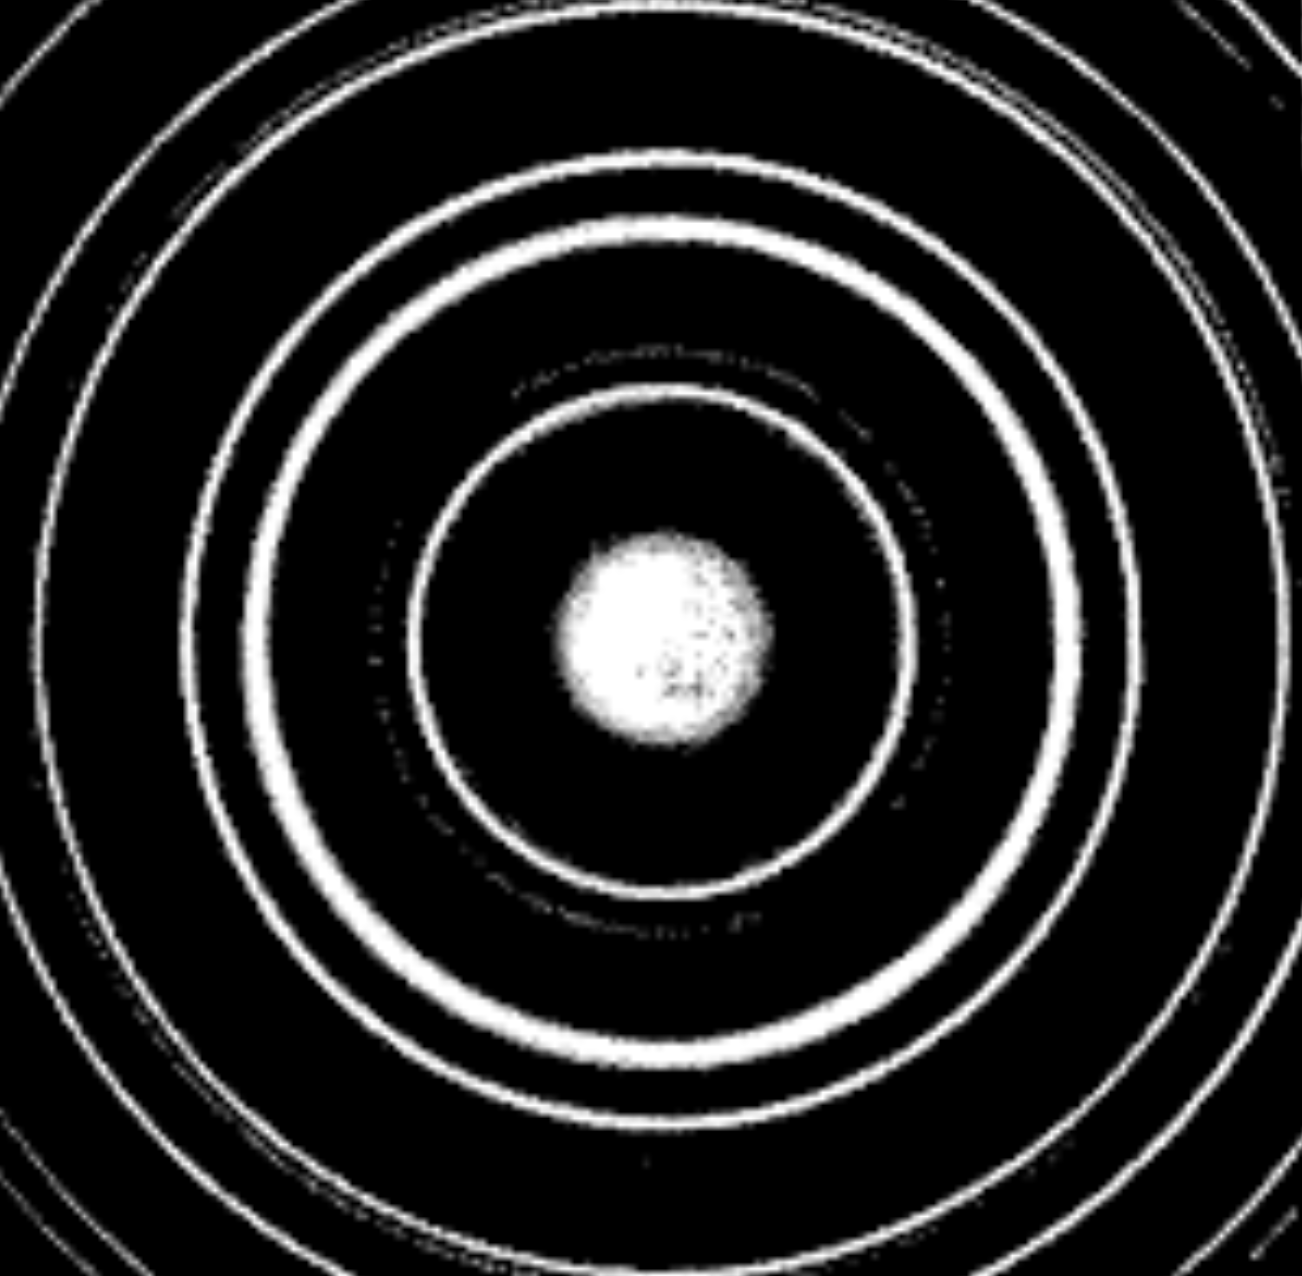
\includegraphics[width=0.8\linewidth]{EDPolyPreferreda.png}
            \caption{Polycrystalline.}
            \label{fig:EDPolyPreferreda}
        \end{subfigure}
        \begin{subfigure}[b]{0.3\linewidth}
            \centering
            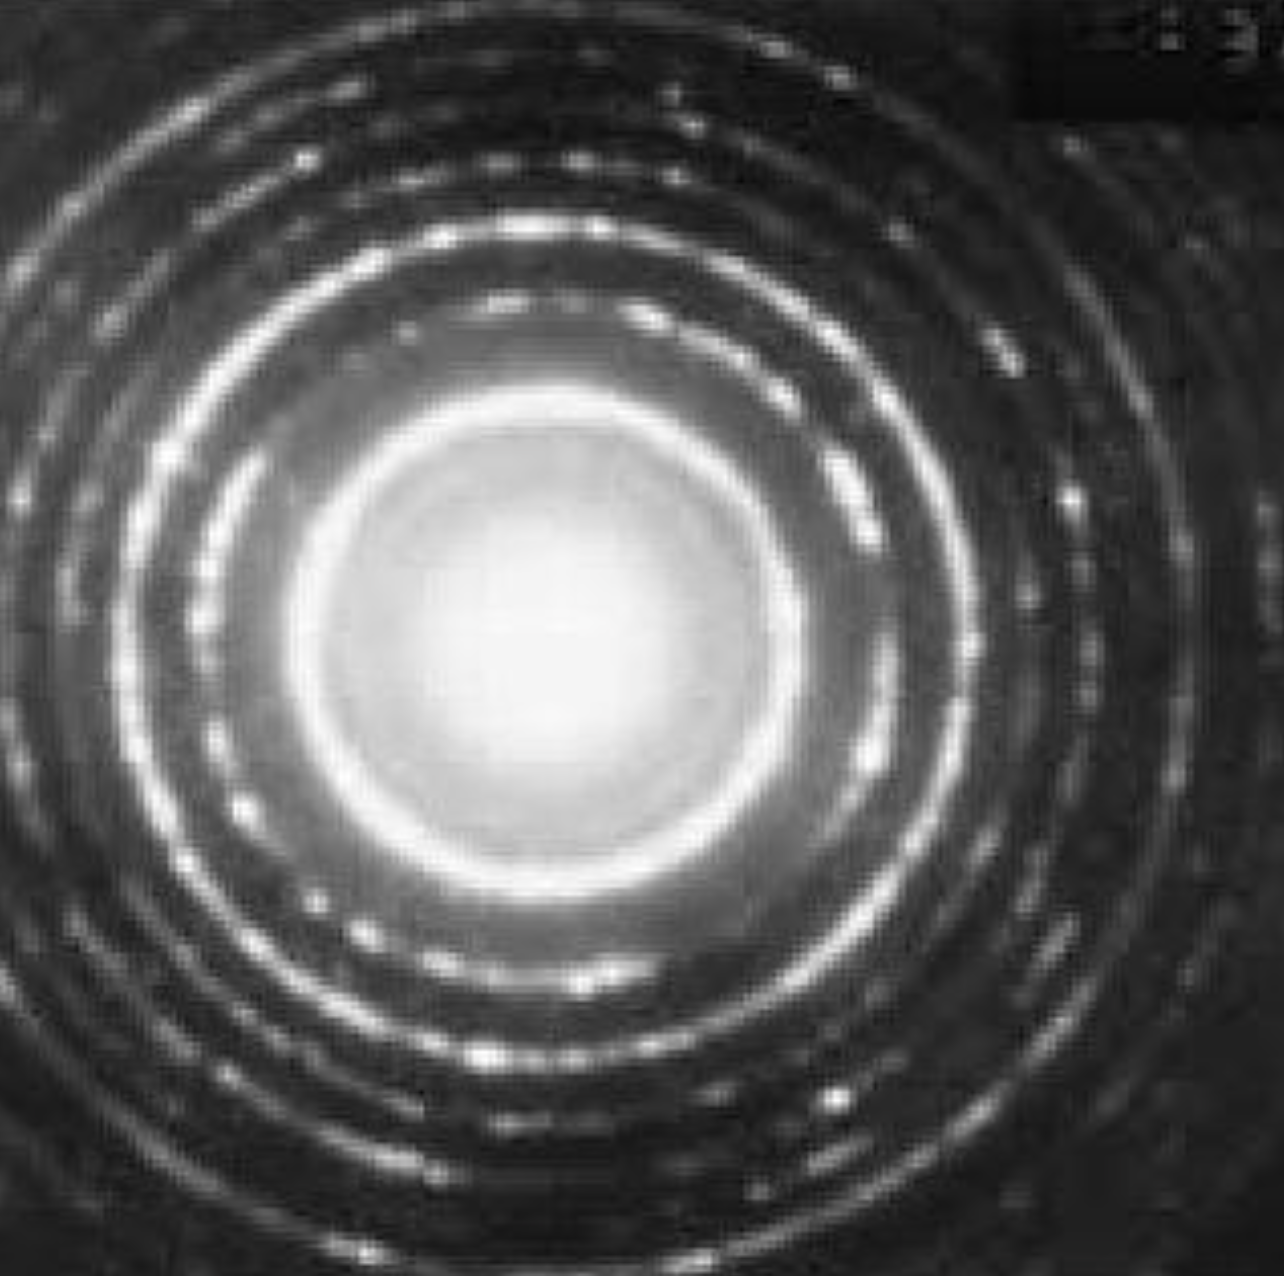
\includegraphics[width=0.8\linewidth]{EDPolyPreferredb.png}
            \caption{Preferred orientation.}
            \label{fig:EDPolyPreferredb}
        \end{subfigure}
        \caption{SAED images of polycrystalline vs. oriented materials.}
        \label{fig:EDPolyPreferred}
    \end{figure}
    \begin{figure}[H]
        \centering
        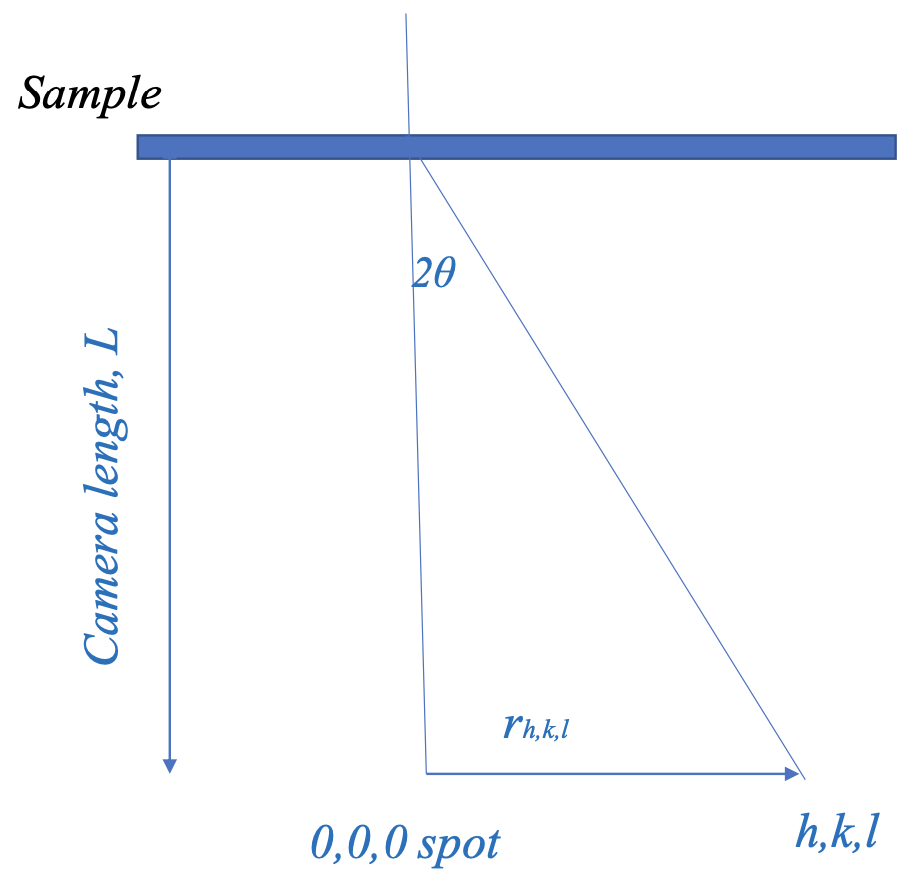
\includegraphics[width=0.35\linewidth]{SAEDDeriv.png}
        \caption{SAED condition derivation.}
        \label{fig:SAEDDeriv}
    \end{figure}
    \begin{itemize}
        \item A \textbf{polycrystalline} material gives perfect circles; each circle corresponds to an $hkl$ plane.
        \item When crystalline domains are in their preferred orientation, the rings appear as broken.
        \item Same diffraction condition as with XRD.
        \begin{equation*}
            \lambda = 2d_{hkl}\sin\theta
        \end{equation*}
        \begin{itemize}
            \item As before, we start with
            \begin{equation*}
                \tan(2\theta) = \frac{r_{hkl}}{L}
            \end{equation*}
            See Figure \ref{fig:SAEDDeriv}.
            \item Moreover, since $\theta$ is very small, we can invoke the SAA. This yields
            \begin{align*}
                \tan(2\theta) &= 2\theta&
                \sin\theta &= \theta
            \end{align*}
            \item Thus, $2\theta=r_{hkl}/L$ and $\lambda=2d_{hkl}\theta$, so
            \begin{equation*}
                r_{hkl}d_{hkl} = \lambda L
            \end{equation*}
            \item $L$ is the camera length.
        \end{itemize}
    \end{itemize}
    \item \textbf{Polycrystalline} (material): A material in which all possible orientations of the crystal domains are present.
    \item SAED example.
    \begin{itemize}
        \item Measuring the distance between the center spot and other spots provides information about the ratios of $d$ spacings.
        \item Not much said on this --- even Shevchenko doesn't know very much about how it works.
        \item Dan Schectman won the 2011 Nobel Prize in Chemistry for results based on this method that he struggled mightily to publish because the scientific community was so skeptical.
        \begin{itemize}
            \item Essentially, he won for the discovery of icosahedral quasiperiodic structure.
            \item The icosahedral symmetry, specifically, of the phase was revealed via SAED.
        \end{itemize}
        \item Outline of Schectman's work.
        \begin{itemize}
            \item Studied the rapid solidification of a melted metal.
            \begin{itemize}
                \item Specifically, he studied the solidified \ce{Al}-\ce{Mn} alloys formed via rapid cooling.
            \end{itemize}
            \item Such cooling leads to the formation of \emph{small-grain polycrystalline microstructures}. These are\dots
            \begin{itemize}
                \item Structures with very small grain sizes;
                \item Extremely difficult to study by X-ray diffraction;
                \item Very suitable for TEM.
            \end{itemize}
            \item The slides have a picture of a series of SAD electron diffraction patterns obtained from the \ce{Al78Mn22} rapidly solidified alloy by tilting a single grain. Based on these patterns, a unique non-crystallographic 10-fold axis and a one-dimensional periodicity of the decagonal phase were established.
        \end{itemize}
        \item For a long time, the community tried to explain away his results as coming from some defect.
        \item Significance: This is the first known example of discovering a particular structure in a manmade material, and only later discovering it in natural materials.
    \end{itemize}
    \item \ce{Au/Fe3O4} nanoparticle superlattices.
    \begin{itemize}
        \item Nanocrystals self-assemble to form a quasicrystal structure.
        \item Image quality improvements are possible via post-processing with mathematical filters, e.g., FFT.
        \begin{itemize}
            \item You have to be careful not to create artificial features in your image, though!
        \end{itemize}
    \end{itemize}
    \item Scanning transmission electron microscopy (STEM).
    \begin{itemize}
        \item Picture of the setup (analogous to Figure \ref{fig:TEMBuildingBlocksb}) present in slides.
        \begin{itemize}
            \item In fact, the only major differences are the addition of deflection scan coils between the condenser aperture and the upper objective polepiece, and the addition of a STEM detector (back focal plane of objective lens) beneath the lower objective polepiece.
        \end{itemize}
        \item Unlike in CTEM, in STEM\dots
        \begin{itemize}
            \item The electron beam is focused to a fine spot (approximate size: \SIrange{0.05}{0.2}{\nano\meter}).
            \item The beam scans over the sample in a raster illumination system that is constructed so that the sample is illuminated at each point with the beam parallel to the optical axis.
        \end{itemize}
        \item STEM is great for analytical techniques such as $Z$-contrast annular dark-field imaging (which we'll talk about later), as well as spectroscopic mapping by energy dispersive X-ray (EDX) spectroscopy and/or electron energy loss spectroscopy (EELS).
        \item A typical STEM is a CTEM plus additional scanning coils and detectors. However\dots
        \begin{itemize}
            \item It can be very expensive to make these modifications, and it can't be done to every instrument.
        \end{itemize}
        \item Addition of an aberration corrector to STEMs enables electron probes to be focused to sub-\si{\angstrom} diameters.
        \begin{itemize}
            \item Images with sub-\si{\angstrom} resolution (better than \SI{1.36}{\angstrom}) can be acquired.
        \end{itemize}
    \end{itemize}
    \item STEM vs. TEM.
    \begin{itemize}
        \item For STEM, there are special requirements for the housing room. To get atomic resolution images in STEM, the level of vibration, temperature fluctuations, electromagnetic waves, and acoustic waves must be limited.
        \item Thus, these machines are usually in a basement in a specially engineered room. Common features include a concrete layer, then some damping polymer, then another concrete layer.
        \item STEMs are also much more complicated-looking, clunky machines. No nice outer shell.
        \item CTEMs are usually built into a workstation with a computer and can be in most any room.
        \begin{itemize}
            \item Is this why GCIS has a sub-basement with all the spectroscopy stuff?
        \end{itemize}
    \end{itemize}
    \item HAADF imaging.
    \begin{figure}[h!]
        \centering
        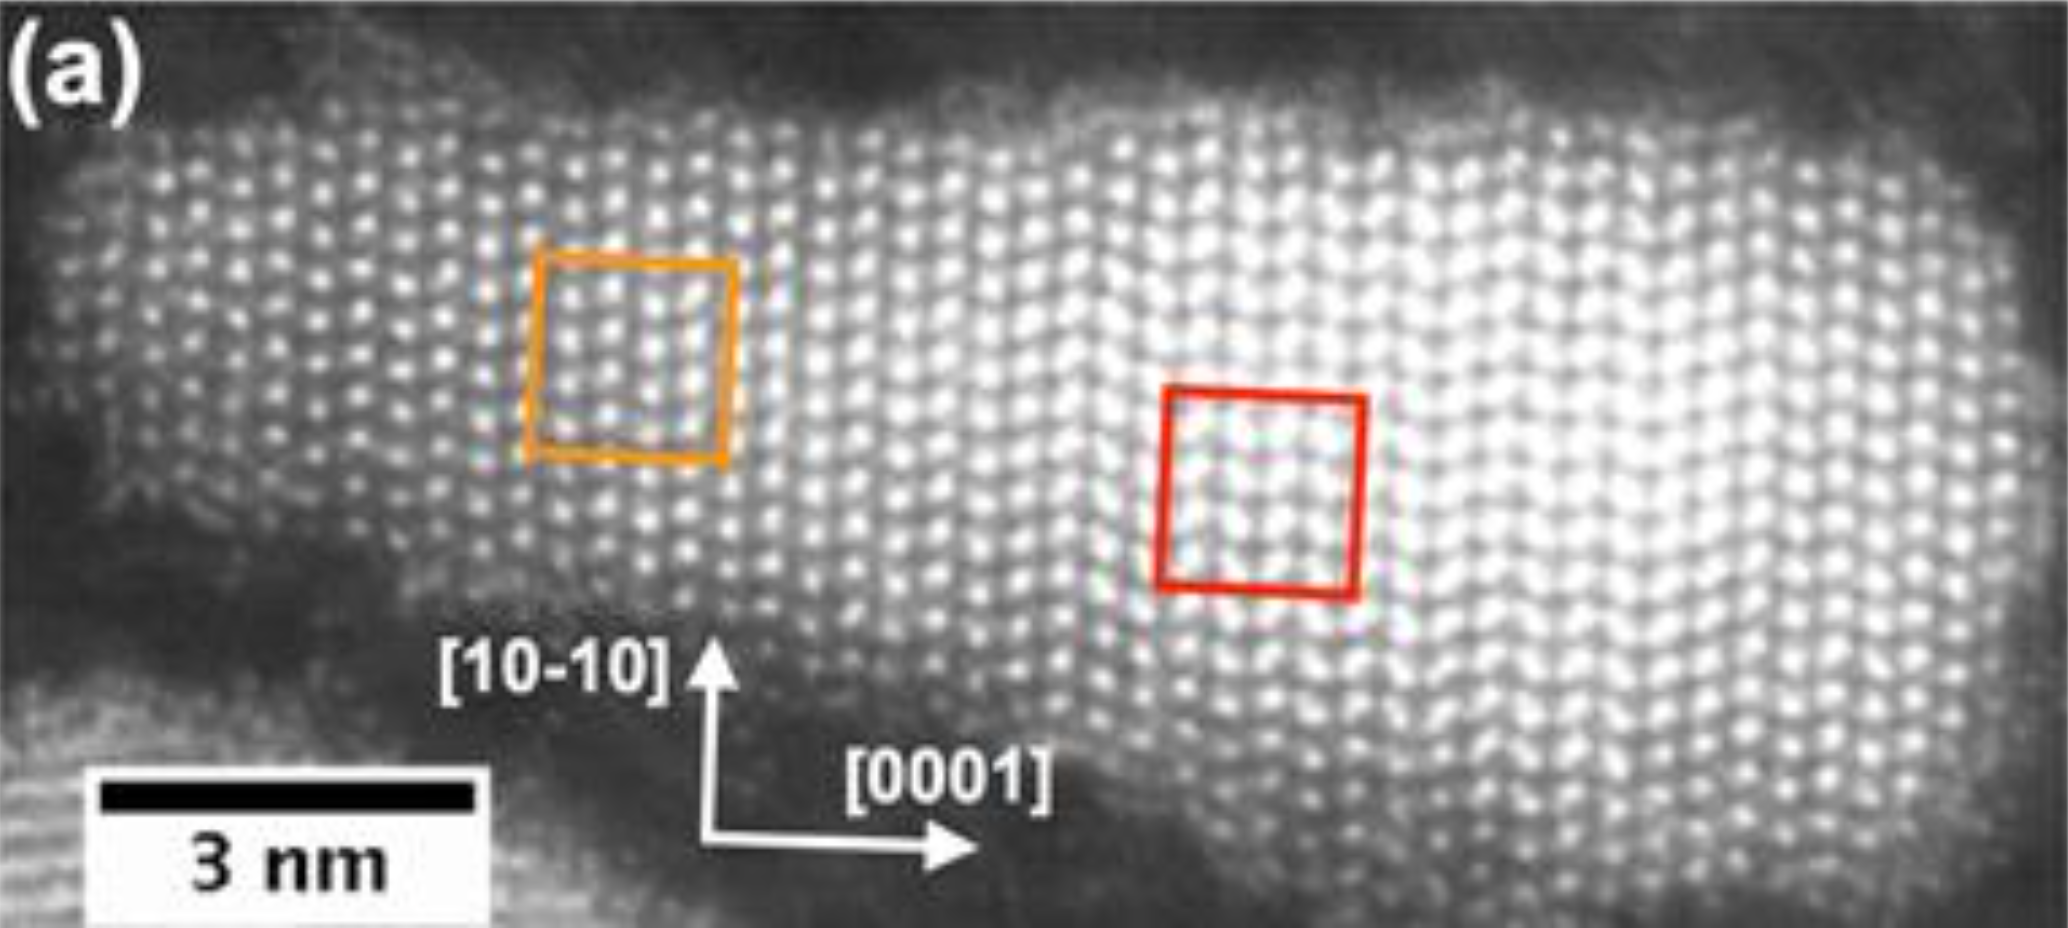
\includegraphics[width=0.4\linewidth]{HAADF.png}
        \caption{HAADF image of \ce{CdSe}/\ce{CdS} nanoparticles.}
        \label{fig:HAADF}
    \end{figure}
    \begin{itemize}
        \item "High angle annular dark field."
        \item The scattering angle and extent of scattering of some electrons depends on $Z$.
        \item The central beam and all electrons scattered at very high semiangle are excluded from imaging.
        \item You block specific scattered electrons.
        \item The HAADF detector enables analysis of the crystals via $Z$-contrast imaging by capturing scattered electrons at specific angles.
        \item The intensity of the scattered electrons at the high angles is proportional to $Z^\alpha$, where $Z$ is the atomic number and $\alpha\in[1.6,1.9]$ for most cases.
        \item Contrast variations in the atomic resolution images can thus be used to delineate the \ce{CdSe} core structure embedded within the \ce{CdS} shell, due to the weaker scattering cross-section of sulfur atoms compared to the selenium atoms.
        \item Orange box is \ce{CdS}, and red is \ce{CdSe}??
        \begin{itemize}
            \item Selenium is brighter, less contrast.
        \end{itemize}
    \end{itemize}
    \item Comparison of CTEM and HAADF.
    \begin{itemize}
        \item In HAADF, significant differences in $Z$ lead to bright spots.
        \begin{itemize}
            \item For example, single \ce{Pt} atoms show up as white circles on an otherwise gray \ce{FeOx} support.
            \item Very much like in Figure \ref{fig:HAADF} with \ce{Se} vs. \ce{S}.
        \end{itemize}
        \item HAADF-STEM imaging is popular in the study of catalysts and electrocatalysts.
        \item CTEM images, on the other hand, just show broader shapes and outlines.
    \end{itemize}
    \item Another HAADF example.
    \begin{itemize}
        \item We can get really high magnification here.
        \item Two layers of \ce{MoS2} on top of each other.
        \item Commentary here on the applications of the FFT to spectroscopy.
    \end{itemize}
    \item Electron energy loss spectroscopy (EELS).
    \begin{itemize}
        \item Picture of the setup (analogous to Figure \ref{fig:TEMBuildingBlocksb}) present in slides.
        \item TEMs contain a great source of electrons for material interactions. However, we don't have to limit these soruces to TEM alone. Indeed, we can repurpose them for other kinds of spectroscopy.
        \item EELS allows you to study the phonons of individual atoms.
        \begin{itemize}
            \item Can also measure oxidation states.
        \end{itemize}
        \item Working principle.
        \begin{itemize}
            \item A sample is exposed to an electron beam with a very narrow energy distribution.
            \item Some electrons undergo inelastic scattering (lose energy and pathways are deflected).
            \item Inelastic interactions include photon excitations, inter- and intra-band transitions, plasmon excitations, ionization of the inner shell, etc.
            \item The \textbf{inner-shell ionizations} are used to analyze the elemental components of a sample and oxidation state.
            \item The amount of energy loss can be measured via an electron spectrometer.
        \end{itemize}
        \item Unless you specialize in microscopy, you won't need to know much about this technique.
    \end{itemize}
    \item Electron tomography.
    \begin{itemize}
        \item It is often the case that a two-dimensional view is not enough; three dimensions is better!
        \item You use special holders that are much smaller and allow more tilting.
        \item Collect images over a large range of tilt angles.
        \begin{itemize}
            \item The more angles, the better the image.
        \end{itemize}
        \item Reconstruct using one of various methods to form a 3D image of the sample.
    \end{itemize}
    \item A "reactor" in TEM: \emph{In situ} TEM.
    \begin{figure}[h!]
        \centering
        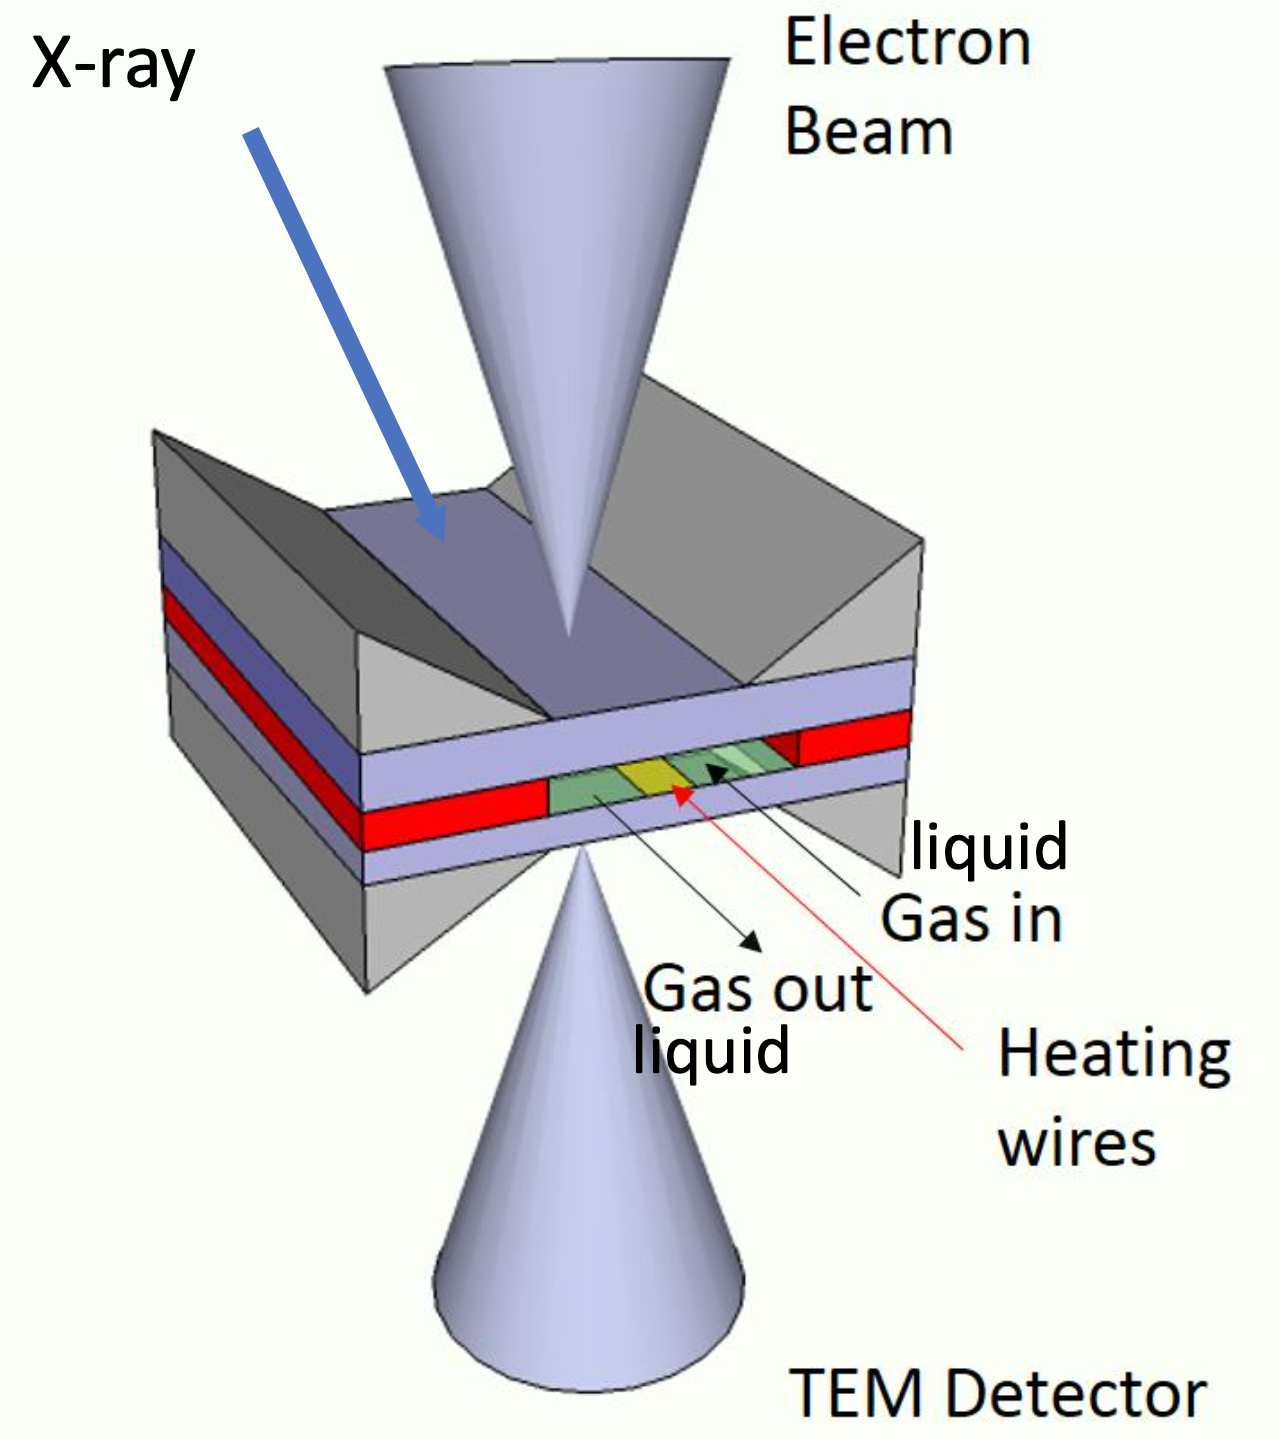
\includegraphics[width=0.25\linewidth]{TEMInSitu.png}
        \caption{\emph{In situ} TEM.}
        \label{fig:TEMInSitu}
    \end{figure}
    \begin{itemize}
        \item There exist special liquid cells that allow you to observe reactions in progress.
        \item You have to be careful to make sure that the electron beam doesn't break the cell --- it's very fragile.
        \item You can also study ion intercalation, which is important to the structural information of battery materials.
    \end{itemize}
    \item Probe the dynamics at atomic scale.
    \begin{itemize}
        \item The atoms at the surface of nanomaterials hop from one position to another based on the electrons.
        \item You can observe atomic rearrangement and stuff like that.
    \end{itemize}
    \item We now move on to X-ray photoelectron spectroscopy (XPS).
    \item XPS is a UHV (ultra-high vacuum) technique.
    \begin{itemize}
        \item Some modifications can enable lower vacuums.
        \item But in general, the higher the vacuum, the better the signal.
        \item Topics of study: Clean surfaces, ambient reactions at surfaces, and controlled adsorption and reaction on clean surfaces, ranging from submonolayer through to situations that go deeper, such as the early stages of oxidation and corrosion.
    \end{itemize}
    \item Contribution of XPS to different fields.
    \begin{figure}[h!]
        \centering
        \begin{tikzpicture}
            \footnotesize
            \pie{
                27/Semiconductor,
                15/Nano-carbon,
                13/Bio-Medical,
                8/Nano-particles,
                8/Polymer,
                7/Thin Film,
                6/Catalyst,
                5/Geology,
                4/Metal,
                3/Adhesion,
                2/Energy,
                2/Other
            };
        \end{tikzpicture}
        \caption{XPS in different fields.}
        \label{fig:XPSFields}
    \end{figure}
    \begin{itemize}
        \item The applications are evidently broad.
    \end{itemize}
    \item How do X-rays interact with matter?
    \begin{itemize}
        \item See Lecture 1.2: Definitions of absorption, elastic scattering, and inelastic scattering.
    \end{itemize}
    \item Photoelectric effect.
    \begin{itemize}
        \item Recall the kinds of electrons that can be generated (Figure \ref{fig:ElectronsMatter}).
        \item To stabilize the atom, an outer shell electron fills the vacancy in the inner shell.
        \item We won't continue to talk about photoelectrons and auger electrons, but recall that the probability of the photoelectric effect is higher when\dots
        \begin{itemize}
            \item The energy of the incident photon is greater than or equal to the binding energy of the electron in its shell;
            \item The electron is tightly bound (e.g., $K$ shell).
        \end{itemize}
        \item Photoelectric absorption is proportional to
        \begin{equation*}
            \frac{pZ^3}{E^3}
        \end{equation*}
        where $p$ is the physical density of the attenuating medium, $Z$ is the atomic number, and $E$ is the energy of the incident photons.
        \begin{itemize}
            \item More on this equation??
        \end{itemize}
    \end{itemize}
    \item X-ray photoelectron spectroscopy.
    \begin{figure}[H]
        \centering
        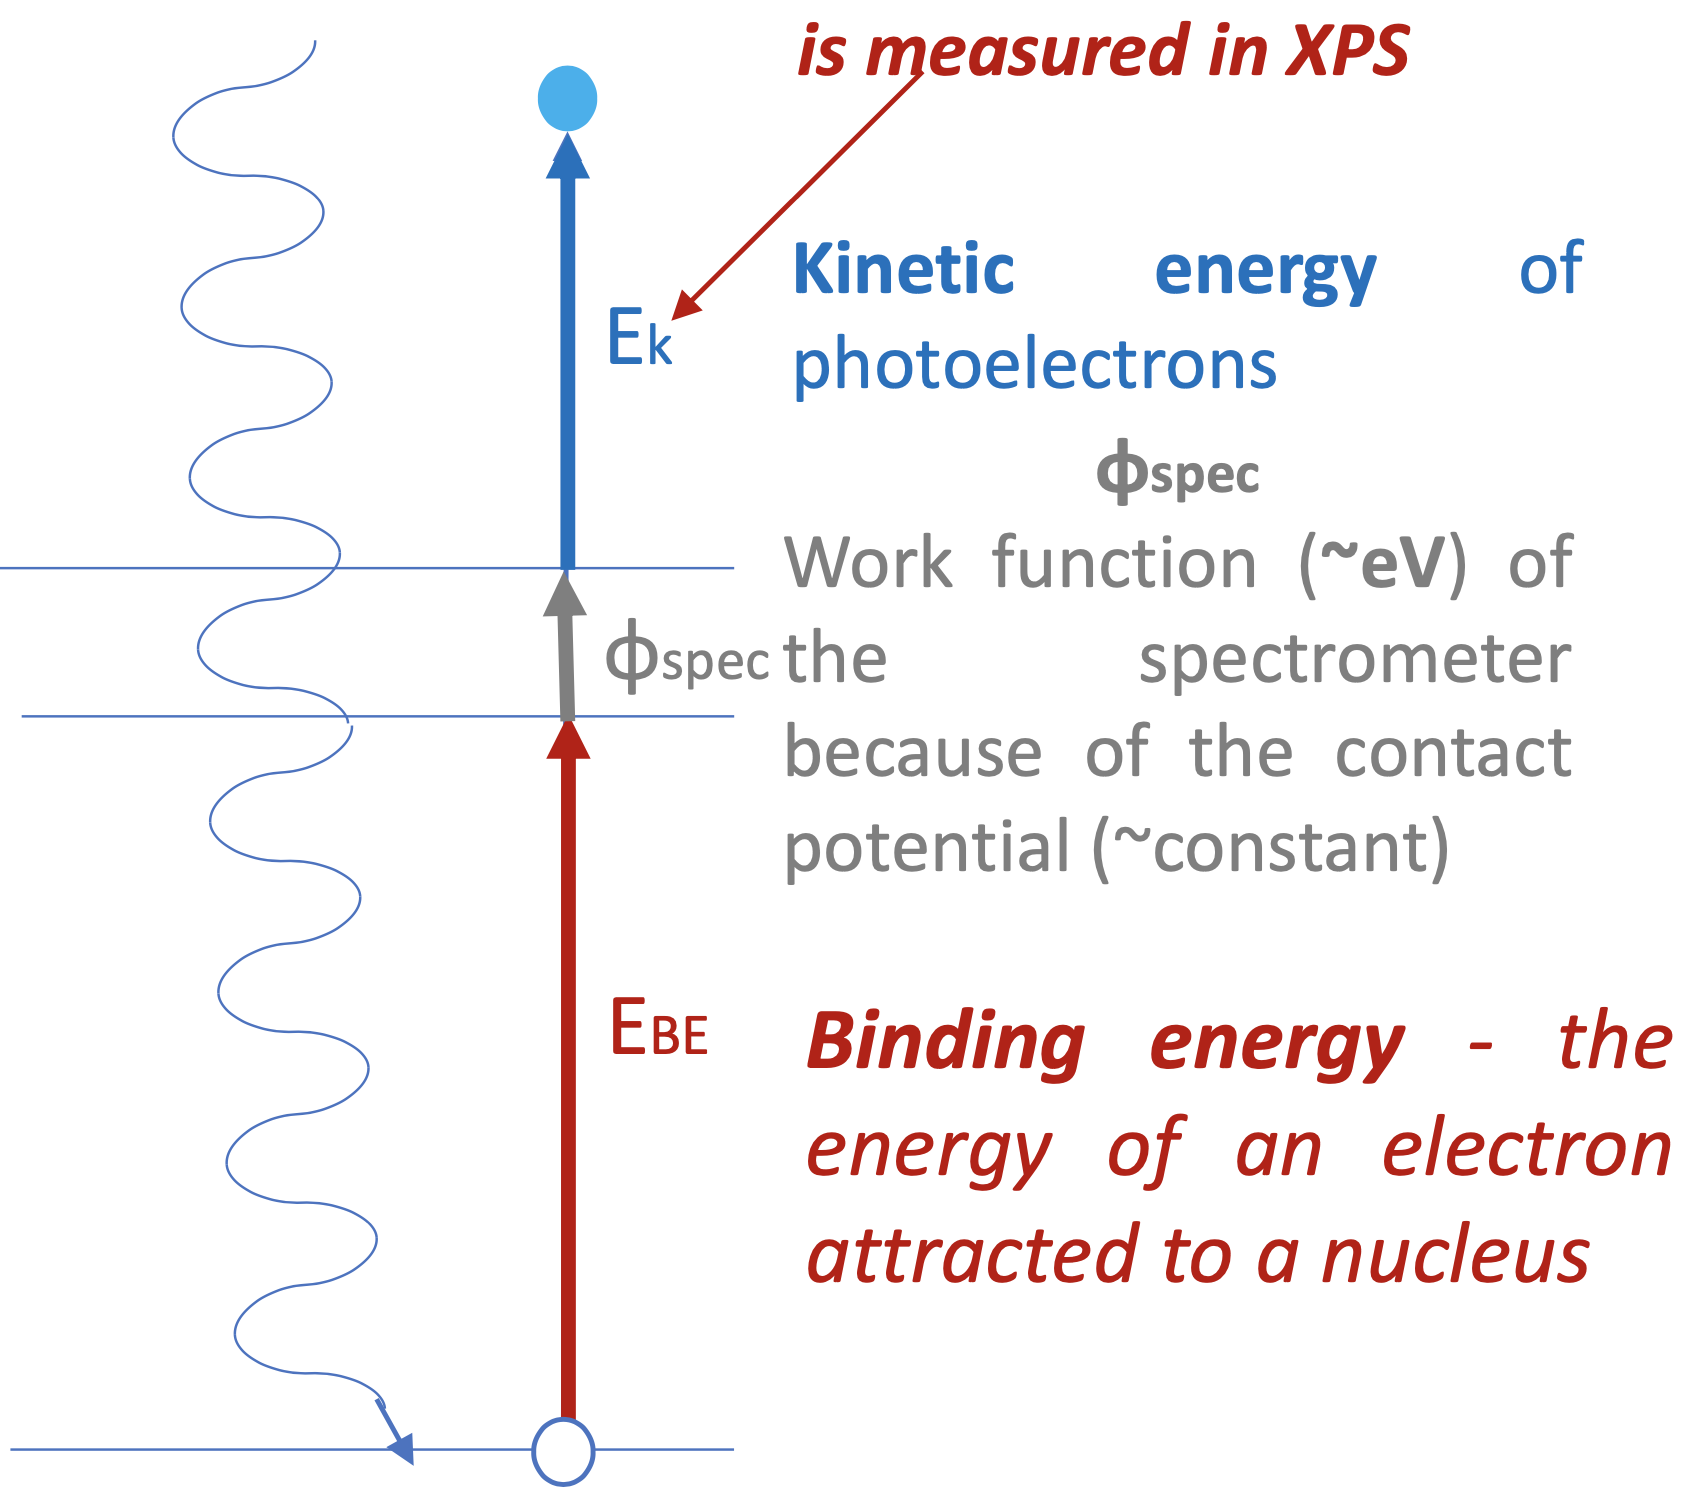
\includegraphics[width=0.35\linewidth]{XPSeqn.png}
        \caption{XPS equation visualization.}
        \label{fig:XPSeqn}
    \end{figure}
    \begin{itemize}
        \item In the domain of XPS, the following equation is very important, but we will not even touch it.
        \begin{equation*}
            h\nu = E_\text{BE}+(E_\text{k}+\phi_\text{sp})
        \end{equation*}
        \begin{itemize}
            \item We want to find out the binding energy $E_\text{BE}$, so we measure $E_k$.
        \end{itemize}
        \item The binding energy tells us how attracted an electron is to its nucleus. In particular, it tells us\dots
        \begin{itemize}
            \item What element;
            \item The valence state of the element;
            \item The coordination environment (e.g., ligands).
        \end{itemize}
    \end{itemize}
    \item Binding energy reference.
    \begin{itemize}
        \item A diagram of how the binding energy works.
        \item Lots of interesting detail, but Shevchenko glossed over it.
    \end{itemize}
    \item Early days of XPS.
    \begin{itemize}
        \item Heinrich Hertz (1887): First experimental observation of the photoelectric effect.
        \item Albert Einstein (1905): Explained the photoelectric effect.
        \item Karl Manne Siegbahn (1924): XPS and Siegbahn notation ($K_{\alpha_1}$, etc.).
        \begin{itemize}
            \item Siegbahn proposed \textbf{Siegbahn notation}; not in common use any more.
            \item There is a chart on it in the slides, though.
        \end{itemize}
        \item Kai Siegbahn (1954): Significant improvements in the equipment; the first high-energy-resolution XPS spectrum of cleaved \ce{NaCl}.
        \item Kai Siegbahn (1967): XPS called Electron Spectroscopy for Chemical Analysis (ESCA).
        \item Kai Siegbahn + Hewlett-Packard (1969): The first commercial monochromatic XPS instrument.
    \end{itemize}
    \item XPS system.
    \begin{itemize}
        \item Schematic of an XPS system (similar to Figure \ref{fig:TEMBuildingBlocksa}, but a real pic).
        \item \ce{Al} $K_\alpha$ and \ce{Mg} $K_\alpha$ provide soft X-rays of \SI{1486.6}{\electronvolt} and \SI{1254.4}{\electronvolt}, respectively.
        \item Why do we need two X-ray sources?
        \begin{itemize}
            \item To separate signals from Auger electrons and photoelectrons: The binding energy does not depend on the energy of the incoming X-rays, but the Augers will be affected.
        \end{itemize}
        \item XPS is not destructive in a classical way; however, it can be coupled with an etching technique that removes the topic atomic layer.
        \begin{itemize}
            \item Can induce possible artifiacts (e.g., induced chemical changes, the preferential sputtering of elements, surface roughening, etc.).
        \end{itemize}
        \item The largest size for a monochromatic beam of X-rays is \SIrange{1}{5}{\milli\meter}.
        \begin{itemize}
            \item Non-monochromatic beam: \SIrange{10}{50}{\milli\meter}.
        \end{itemize}
        \item XPS with synchrotron radiation: Down to $\sim\SI{200}{\nano\meter}$.
    \end{itemize}
    \item Survey XPS spectra.
    \begin{itemize}
        \item This is the first step; scan in a broad energy range. This will allow you to identify all elements present in the sample.
        \item Drop and dry on a silicon wafer.
        \item Wide-scan survey spectrum showing all elements present.
        \item Then narrow the range for high-resolution XPS spectrum.
    \end{itemize}
    \item XPS spectra: Example.
    \begin{itemize}
        \item A series of oxide films of \ce{Ni}-\ce{Cr}-\ce{Mo} alloys (corrosion resistant alloys in both oxidizing and reducing environments).
        \item The spectra are usually presented from higher to lower counts; this is just canonical.
    \end{itemize}
    \item Alex Filatov is a great resource for questions on XPS; Shevchenko only does it from time to time.
    \item Analysis.
    \begin{itemize}
        \item Three main things.
        \begin{enumerate}
            \item Peak position (along the $x$-axis, which is binding energy in \si{\electronvolt}): Indicates the elemental and chemical composition.
            \item Peak intensity ($x$-axis, total number of photoelectron counts per second): Indicates how much of a given element is present at a sample's surface.
            \item Overlapping peaks (complication; \ce{Sn} and \ce{Pb} can have interfering peaks).
        \end{enumerate}
        \item XPSPEAK4.1 is an open-source peak fitting software that Shevchenko recommends.
        \begin{itemize}
            \item CASA is a powerful, reliable, and broadly used software.
        \end{itemize}
        \item Make sure to check tables from multiple sources!
        \item The number of peaks produced by a single element varies from 1 up to many.
    \end{itemize}
    \item XPS signals.
    \begin{itemize}
        \item Ideal case is no background.
        \begin{itemize}
            \item All the intensity is from photoionizing a $1s$ electron of \ce{Li} and a $1s$ electron from \ce{F}.
            \item No contribution of instrumental correction (work function).
            \item Relative atomic concentrations: The measured intensities (the areas under the peaks) normalized by a partial photoionization cryss section $\sigma$.
        \end{itemize}
        \item However, we often have some extrinsic background.
        \begin{itemize}
            \item Formed from Auger electrons.
            \item Peaks are formed by the intrinsic electrons ejected through the \ce{LiF} matrix without energy loss (inelastic scattering). The inelastic mean free path length is very small, so the peaks originate from the surface.
            \item The background is from photoelectrons that underwent inelastic collisions and lost energy on the way out (the extrinsic photoelectrons scattered once, twice, etc. times --- energy contribution over a broad range ---- the background step extends 100s eV to lower KE).
        \end{itemize}
    \end{itemize}
    \item Probability of the electron transitions.
    \begin{itemize}
        \item Intensity ratio is given by
        \begin{equation*}
            \frac{2j_-+1}{2j_++1}
        \end{equation*}
        \begin{itemize}
            \item $j$ is the quantum number $j=l+s$.
        \end{itemize}
        \item The relative photoelectron peak intensities are determined by the relative probability (partial photoionization cross sections) for each orbital level to undergo photoionziation at given $h\nu$.
        \begin{itemize}
            \item These depend on the overlap between the X-ray wavefunction and the orbital wavefunction.
        \end{itemize}
        \item Why can't \ce{H} and \ce{He} be detected by XPS?
        \begin{itemize}
            \item All electrons are used in chemical bonds; and the cross section is extremely low.
            \item Are bonding electrons generally harder to knock out than atomic ones??
        \end{itemize}
    \end{itemize}
    \item Example: U.
    \begin{itemize}
        \item A plot of the relative binding energies and ionization cross-section for uranium.
    \end{itemize}
    \item \textbf{Spin orbital coupling}: The distance between the two peaks.
    \begin{itemize}
        \item The values of spin orbital splitting of a core level of an element in different compounds are nearly the same.
        \item The \textbf{peak area ratios} of a core level of an element in different compounds are also nearly the same.
        \item For $p,d,f$ peaks, two peaks will be observed.
    \end{itemize}
    \item \textbf{Chemical shift}: A slight change in the binding energy of a core electron due to major changes in the valence levels.
    \begin{itemize}
        \item Caused by bonding between atoms (chemistry --- oxidation and coordination).
        \item Core binding energies of the electron depend on the electrostatic interaction between it and the nucleus.
        \item Core binding energies of the electron can be reduced by the electrostatic shielding of the nuclear charge from all other electrons in the atom, including valence electrons.
        \item Withdrawal of valence electrons (e.g., oxidation) leads to an increase in binding energy.
        \item Addition of valence electrons decrease the binding energy.
        \item Gold need not be 1 or 3; it can also be partially shifted.
        \item Binding energy in oxides is higher because electron density (e.g., $2s$) can be transferred to oxygen.
    \end{itemize}
    \item Background.
    \begin{itemize}
        \item How do we edit out the background?
        \item Simplest method: Draw a straight line between the beginning and the end of the peak.
        \begin{itemize}
            \item The area under the peak is almost unaffected by small variations in where one picks the start and end.
            \item Good for qualitative analysis, not for quantitative analysis.
        \end{itemize}
        \item Shirley background subtraction requires picking start and finish points, and the background goes up in proportion to the total number of photoelectrons below its binding energy position.
        \item Tougaard background subtraction is not entirely empirical, and attempts to calculate the actual inelastic scattering events used parameters derived from other experiments.
        \item There are also others.
        \begin{itemize}
            \item Ask Filatov if you're still curious; it's a good question for him.
        \end{itemize}
    \end{itemize}
    \item Satellite features.
    \begin{itemize}
        \item Some of the photon energy can be used to excite the ion out of the zero loss state while at the same instant ejecting the photoelectron with the remaining photon energy. Example: Shake-up structure in the $2\rho 3/2$ spectrum for \ce{Cu^{II}} species in \ce{Cu(OH)2} and \ce{CuO}.
        \item Shake-off events when more than one electron is ejected at the time of photoionization may lead to broadening of the core level peak.
    \end{itemize}
    \item XPS on insulating materials.
    \begin{itemize}
        \item Surface charge buildup: Positive charge at or near the sample surface is built up due to the emission of electrons. This charge build up can be non-uniform and can shift the energy of photoelectrons emitted from the sample, distorting the peak shape.
        \item Siegbahn method relies on the use of \ce{C}($1s$) spectra of \textbf{adventitious} carbon present on all surfaces exposed to the ambient air (\ce{C-C}/\ce{C-H} component of the measured \ce{C($1s$)} spectrum has a binding energy in the range of \SIrange{284.6}{285.0}{\electronvolt}; the $\Delta_\text{corr}$ is determined from the measured peak and applied as a constant shift to all peaks in the spectrum).
    \end{itemize}
    \item No exam questions on any of the following.
    \item X-ray fluorescence (XRF).
    \begin{itemize}
        \item XRF basics.
        \begin{itemize}
            \item The energy of X-ray fluorescence photons is characteristic of each element.
            \item XRF is quantitative, i.e., the number of XRF photons is directly related to the quantity of the element.
            \item The photoelectric effect absorption crosssection is simple to calculate (use a monochromatic incident beam).
        \end{itemize}
        \item Spectroscopy that takes advantage of XRF: EDXRF.
        \begin{itemize}
            \item Energy dispersive X-ray fluorescence (EDXRF) is a routinely used analytical technique for the qualitative and quantitative determination of major and minor atomic elements in a wide variety of sample types.
            \item Rapid, non-destructive, multi-element analyses from low ppm levels to high weight percent (wt\%) concentrations.
            \item Non-destructive analysis of sodium to uranium in almost any matrix, from oils and liquids to solids, metals, polymers, powders, pastes, coatings, and thin films.
        \end{itemize}
        \item Applications.
        \begin{itemize}
            \item Especially well-suited for semi-quantitative determination of elemental content in complete unknowns.
            \item The instrument has variable spot size to collect information from different areas.
        \end{itemize}
    \end{itemize}
    \item X-ray fluorescence at a synchrotron.
    \begin{itemize}
        \item We need: A coherent and monochromatic X-ray beam, optics, a sample mount, and a detector to read the spectrum.
        \item Schematic of a hard X-ray microscope.
    \end{itemize}
    \item XRF at APS.
    \begin{itemize}
        \item A few sample mount options (described in the slides).
        \item The beam size in Sector 2 is \SI{450}{\nano\meter} and the step is \SI{200}{\nano\meter}.
    \end{itemize}
    \item Investigation of cartilage.
    \begin{itemize}
        \item Pretty straightforward application ow what came before.
    \end{itemize}
    \item Bench-top XRF instruments.
    \begin{itemize}
        \item A \SI{60}{\kilo\volt} X-ray tube for wide elemental coverage (typically).
        \item Automatic sample changers, sample spinner, and helium purge or vacuum atmosphere.
    \end{itemize}
    \item Reading recommendation.
    \begin{itemize}
        \item These provide great overviews of what we've talked out and what can be used to provide answers about various types of nanomaterials.
    \end{itemize}
    \item Shevchenko will share last year's exam and this year's will be simpler; solve all questions.
\end{itemize}



\section{Hands-On Class}
\begin{itemize}
    \item \marginnote{1/26:}XPS at this school never works.
    \item Taught by Sophie Anferov (formerly Whitmeyer).
    \item Sophie runs a lot of samples for a lot of people. Dong and Levin group have trained crystallographers, but most people go through her.
    \item Sophie is a 4th year and will be thinking about passing the job along soon, so if we're interested, we should reach out.
    \item If we ever have crystals (we're not organic, so probably not many of us), we can email Alex and CC her; they have a crystallography form that you can submit and then they'll schedule you.
    \item First, we have to crystallize them.
    \begin{itemize}
        \item Use a solvent that your substance isn't readily soluble in and pull your crystal out or add another solvent to kick it out; you want to promote slow growth.
    \end{itemize}
    \item Crystals are special because of their periodicity.
    \item Most crystals are run cold ($\sim\SI{100}{\kelvin}$ here and in a \ce{N2} stream).
    \begin{itemize}
        \item It shouldn't ice, but if you ever do see icing, let them know; it will affect your results since ice is a crystal, itself!
    \end{itemize}
    \item Crystals are run overnight (4PM-next morning) to get as much data as possible.
    \item This instrument has a molybdenum source for most crystals (90\% of the time; goes out further, better bond resolution, and bright enough) and a copper source for some (you need brighter, but will not "go out as far"). If you get a chiral space group, switching to copper may make sense.
    \item This diffractometer model is 8-10 years old, but Sophie thinks its one of the best ones since some newer ones have problems.
    \item The copper and molybdenum X-ray tubes are on the right.
    \item This facility is mainly single crystal (the only one on campus), but can also do some PXRD.
    \item The doors need to shut for the X-ray to turn on; make sure they're shut if you're having errors!
    \item There is an emergency eject switch on the inside, but obviously don't get trapped inside.
    \item Lights on the left side mean that both beams are ready to go.
    \item \textbf{Twin spectra}: The dual spectra of two crystals overlaid on top of each other; complicates your results.
    \item Crystals with lines in them are not good (inspect in dark mode on the microscope); this probably means they have a crack or an impurity.
    \item "It's nice to have something you know diffracts in case something weird is happening."
    \item We put the crystals in mineral oil to get them here, and then get them into the machine with a \textbf{crystal loop}.
    \begin{itemize}
        \item Our loops are made of plastic (amorphous and thus don't show up) and glass.
        \item There's a lot of loop history, but Sophie isn't familiar.
    \end{itemize}
    \item Your goal in mounting a crystal is to get the crystal onto the tip of the loop; it needs to be well-centered.
    \begin{itemize}
        \item This is a bit of an acquired skill.
        \item If you don't center it properly, it may move out of the field during a rotation in the experiment.
        \item The beam lies in the top-right quadrant, not the center, so you have to put it there.
    \end{itemize}
    \item Make sure that the distance is about twice the length of your longest plane; if you have 10,10,20, then use 40??
    \item Mineral oil helps it adhere to the loop, helps with air sensitivity, and prevents things from skittering away if you...
    \item If your compound is soluble in Pet ether, it will probably dissolve in the mineral oil, in which case you need to use very small quantities of oil and move quickly. There aren't really many alternatives to oil, so you just have to be fast.
    \item An intense ring indicates a powder structure; we need to watch out for this.
    \item You can take sample scans.
    \begin{itemize}
        \item Here, our first step is determining the unit cell; this is an important check to make sure that our compound looks right. Prevents us from wasting our money and time on an XRD experiment.
        \item This is not necessary at Argonne (or other synchrotrons), though.
    \end{itemize}
    \item Most analysis is done on the new computer in the room.
    \begin{itemize}
        \item Has a nice Cambridge database downloaded.
        \begin{itemize}
            \item The CCDC.
            \item Nicer than what you can get online.
        \end{itemize}
        \item Unit cell search to start.
        \item It's best policy to submit structure to the database before/after publishing. All of the information you need to upload should be in your crystal file. Questions? Ask Alex or Sophie.
    \end{itemize}
    \item They \emph{can} collect \textbf{connectivity structures} (lower res), but usually they only collect publication-quality structures.
    \begin{itemize}
        \item Certain organic professors like publishing low-res structures, but this makes the department look bad.
    \end{itemize}
    \item You need to make sure that every frame in a rotation video has spots in it.
    \item Sensitivity around 5 to collect lots of spots, but not spurious ones. Then click harvest. 51 distinct spots is usually enough to get a unit cell.
    \item Some people don't use least squares, but Sophie thinks its fine. Least squares and other mathematical techniques help you solve the structure.
    \item Any time you see "rhombohedral" or "cubic," you may well be running a salt.
    \begin{itemize}
        \item They always run in triclinic.
    \end{itemize}
    \item They charge for a more expensive first hour and much less expensive consecutive hours to encourage collecting good data.
    \item To confirm the unit cell, you want to make sure that the dots show up as a grid.
    \item The database allows us to make sure that our crystal isn't something common.
    \item We size the crystal from a video that we take.
    \begin{itemize}
        \item Nice to take the video before collection in case something happens to your crystal during the experiment.
    \end{itemize}
    \item Molybdenum's quality cutoff is \SI{0.84}{\angstrom}; if you have a lot of difficulties, you can sometimes get results up to \SI{0.9}{\angstrom} published. Above that is a connectivity structure.
    \item Quick solve from connectivity data is about 100 frames; if it's not what you want, then adjust.
    \item There are a bunch of strategy parameters to adjust.
    \item Hang out for the first 10 frames and then leave, come back the next morning and do your data analysis.
    \item Data workup is done in Apex.
    \begin{itemize}
        \item Sophie goes through a worked example.
    \end{itemize}
    \item Any correlation above 0.5 is good, 0.3-0.4 may be solvable, below that leads to issues.
    \item Twin solves can be done, but it's a lot more work. You may not always be able to grow distinct crystals.
    \item Look for clean spots, no rings, and no twins.
    \item Scaling is different in different places (Argonne doesn't use an absorbance correction for instance).
    \item Cut the data around 30-50.
    \item After Apex, use Xprep.
    \item The software's suggestions are usually fine, even though we don't have to take them.
    \item Make sure your minimum $I/\sigma$ stays above 2. Completion shouldn't go below 90\% if you want to publish.
    \item The worse your data is, the better your guess must be.
    \item If fixing really isn't working, you may need to do \emph{something more}.
    \item "Never trust someone who says they know where protons are."
    \begin{itemize}
        \item They're too low $Z$.
    \end{itemize}
    \item If your research ever really depends on an \ce{OH} or \ce{NH}, you need alternate data.
    \item \ce{CH3}'s and \ce{CF3}'s have free rotation.
    \item Crystal data is almost always a solid-state analysis; we can't make claims about how our molecule behaves in solution based on the crystal data.
    \item A cool application of symmetry things from group theory, very puzzley, and you get to work with actual molecules instead of powders.
\end{itemize}




\end{document}